\chapter{Semantic Web Practice} \label{ch:semanticwebpractice}

This chapter studies the design, development and deployment of ontology and semantic web model. Both the methodologies and the tools are concerned.

\section{Ontological Engineering}

Different ontologies (class, property, hierarchy, interpretation, logic, etc.) can be used to describe the identical knowledge. This is known as the ``problem of semantic gap''. It is challenging (maybe impossible) to find the optimal and consistent way of representing the knowledge using ontology and semantic web. 

Ontological engineering studies the systematic ways to design the ontology and the semantic web for a specific domain, application or task (recall Fig. \ref{fig:ontologylevel}). It has at least the following research interests:
\begin{itemize}
	\item Ontology design concerns with the methods to systematically design, develop, and develop ontology models.
	\item Ontology mapping concerns with the methods to efficiently compare different ontology models.
	\item Ontology merging concerns with the methods to efficiently combine ontology models.
	\item Ontology learning concerns with the automatic learning of new knowledge by an existing ontology model, when new data sets are provided.
\end{itemize}

\section{Ontology Design}

Ontology design describes all activities necessary for the construction of an ontology model. The goal is to design ontology models efficiently, consistently, and sometimes distributively (collaboratively) if required. Notice that a good ontology model is not built in one go. It is often iteratively improved. 

\subsection{General Tasks}

Design, develop and deploy ontology model for a sophisticated system can be time and manpower consuming. It is important to manage each step during the entire procedure to ensure healthy development of the system. This includes
\begin{itemize}
	\item Scheduling: identify tasks and problems to be solved by the semantic web; plan and arrange resources, time, manpower and money ahead.
	\item Control: guarantee correct execution of tasks and problems to be solved.
	\item Quality assurance: guarantee all steps are done correctly, including using the correct software, and everything is documented in details.
\end{itemize}

In pre-development stage, environment study needs to be carried out. This is mainly to identify what software to use to host the semantic web, and what interface/API shall the semantic have, and what applications would call the API to talk to the semantic web. A feasibility study is also necessary. For example, we need to consider whether it makes sense to develop a semantic web for the application, and whether the semantic web design is realizable.

In development stage, domain expert needs to come in to build domain knowledge in a conceptual model. Knowledge engineer or data scientist then formalize the conceptual model into a computable (formal) model, then into ontology representation language.

Finally, in the post-development phase, pipeline needs to be designed to maintain, update and scale up and down the ontology model. In the case where the ontology model needs to be migrated into different platforms, used by unplanned applications, or merged with other models, necessary changes need to be made to the model. In the case when the knowledge in a model needs to be exported, knowledge recycle needs to be supported. 

There are many ontology support activities. These activities need to be carried out during the different stages of ontology development. Below is a list of some of these activities.
\begin{itemize}
	\item Knowledge acquisition. Interview experts in the field and learn domain knowledge from them. This is referred as ontology learning. This is often done manually by the knowledge engineer or data scientist in the beginning stage. It is also possible to develop tools to automatically gather information and transfer it into ontology models, and even merge it with existing models.
	\item Technical evaluation. A domain expert checks the developing ontology model occasionally to make sure everything is correct.
	\item Integration and merging. This refers to the case where a big (scaled-up) ontology model can be built from a small existing ontology model.
	\item Alignment. Where there are multiple ontology models describing the same physical thing, alignment needs to be made to ensure knowledge consistency.
	\item Documentation and version management.
\end{itemize}

\subsection{Ontology Design Basics} \label{subsec:ontology_design_basics}

Designing comprehensive ontology model and associated semantic web requires professional skills from knowledge engineers and data scientists. In this section, a basic method is introduced for tutorial purpose. The method introduced in this section, like many other ontology design methods, involves the iterative designing and refining the model.

If there is an expert from the domain of interest, discuss with him each step during the design.

\vspace{0.1in}
\noindent \textbf{Determine the Scope}
\vspace{0.1in}

As a first step, decide what knowledge should be included in the semantic web. It is important to draw a clear boundary between what the ontology should include, and what should not.

Decide what the ontology would be used for, who would use it, and what kind of information the user needs to query from the ontology model. Think of a list of competence questions, i.e., the questions that the semantic web would be asked in its practical usage.

Notice that the scope of the ontology model, especially the competence questions may change during the development of the semantic web. Try to leave some margin and look at the bigger picture.

Look for existing ontology model of similar scope, and consider reusing them instead of starting from scratch whenever possible. This should same the cost. In addition to the semantic web itself, the interface, add-on tools, etc., can also be reused.

\vspace{0.1in}
\noindent \textbf{Determine the Vocabularies: Symbols and Interpretations}
\vspace{0.1in}

As the first step to design the schema of the semantic web, it is often a good idea to brainstorm the symbols and interpretations the semantic web would want to include as part of the knowledge base.

For example, to build a semantic web for fruits, visit a local store and list down all the fruits on sale on a piece of paper, as well as the food that goes well with the fruits. This would often serve as a good starting point.

If the domain of interest already has a database (not necessarily semantic web), let the existing data stored in the database to inspire the ontology design. The data usually reflects the features that people concerns with the most, and they shall probably be covered in the semantic web as well.

\vspace{0.1in}
\noindent \textbf{Design Hierarchy and Associate Properties}
\vspace{0.1in}

Once we have a big picture of what symbols and terms to be included in the semantic web, go through the vocabularies and categorize them into classes, relations and properties. Design class and property hierarchies accordingly. 

Furthermore, associate properties with classes, i.e., decide the domain and range of properties as well as the constraints.

\vspace{0.1in}
\noindent \textbf{Populate Classes with Individuals}
\vspace{0.1in}

Finally, once the schema is ready, populate the classes with individuals, and assign properties to these individuals. The individuals may come from an existing database, in which case information conversion is required. A program that automates the information conversion would become handy when the amount of data is huge.

\vspace{0.1in}
\noindent \textbf{Iterative Development}
\vspace{0.1in}

Notice that the above processes shall be carried out iteratively to improve the ontology model and the semantic web. 

\subsection{Semantic Web Design for Enterprise}

The basic semantic web design method introduced in Section \ref{subsec:ontology_design_basics} is not suitable for large size enterprise tier semantic webs, in the later case of which a more formal workflow is often required. Continuous inputs from domain experts and knowledge engineers are expected.

An demonstration of the workflow is given in Fig. \ref{fig:swdesignwf}.
\begin{figure}[htbp]
	\centering
	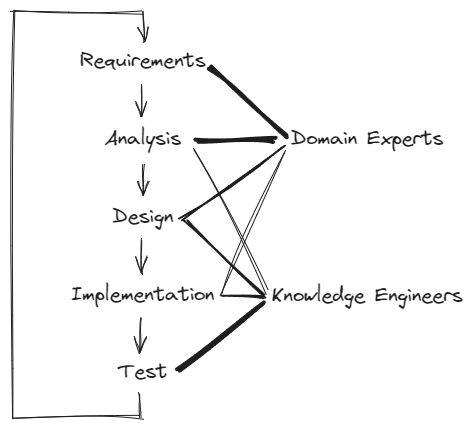
\includegraphics[width=0.6\textwidth]{./chapters/ch-semanticwebpractice/figures/semantic_web_design_workflow.png}
	\caption{Semantic web design workflow.}
	\label{fig:swdesignwf}
\end{figure}
In the workflow, domain experts and knowledge engineers get different involvement at different stages of the workflow. The workflow is iteratively executed for many times, each time with a different focus. For example, in an early stage of the design, an iteration may focus on the lexicon of the semantic web, while in an late stage, on OWL.

There are existing ontology ``templates'' available in the community. These templates are essentially reusable ontology models one can learn from and adapt to his application as a starting point. An repository of such templates is given in 
\begin{lstlisting}
http://ontologydesignpatterns.org/
\end{lstlisting}

\section{Linked Data Engineering}

Linked Data is a set of design principles for sharing machine-readable interlinked data on the internet. Linked Data engineering, as its name suggests, is the practice of creating, managing and sharing machine-readable (and also human readable, in most occasions) data on the web.

\subsection{Web of Data}

Consider the conventional way of retrieving data from a web server as shown in Fig. \ref{fig:webbrowsing}. The address of the server, in this case a URL, is used to identify the server. The local machine request for services using the web API defined by the server. HTTP/HTTPS protocol is used to shake hand and transmit the data between the server and the local machine. Behind the screen, the server retrieves the data either from other web servers or from its internal database.
\begin{figure}[htbp]
	\centering
	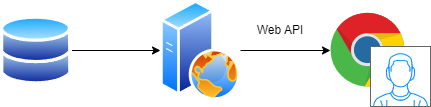
\includegraphics[width=0.6\textwidth]{./chapters/ch-semanticwebpractice/figures/webbrowsing.png}
	\caption{Linked Data example: web browsing.}
	\label{fig:webbrowsing}
\end{figure}

A web server is like an isolated data island. Different web servers may apply different web APIs. The web API decides what services the server provides as well as how the local machine can interact with the server. When a server changes its web APIs, all applications linked to the server also need to change the associated interfaces. 

In addition, since the servers are isolated both physically and logically, it is difficult for the local machine to retrieve, compare and process semantically relevant data across machines. This is certainly a drawback as the data retrieving and processing would have been more efficient and reliable if the data is linked together from the semantic perspective.

Linked Data tries to address the above issues by standardize the way data is stored and shared. Some important principles include:
\begin{itemize}
	\item Use (HTTP) URIs as the names for information pieces. URIs are standardized and both human and machine readable. When HTTP URIs are used, people can conveniently access the information pieces and look up things.
	\item Use RDF to store information, and support SPARQL for querying information. This adds semantics, flexibility and scalability to the information.
	\item In each knowledge piece, include links (in the form of URIs) to other knowledge pieces. This allows linking information pieces together, though they might be stored physically distributively.
\end{itemize} 

As an example, the following is the URI to HTML page of ``William Shakespeare'' on DBpedia.
\begin{lstlisting}
https://dbpedia.org/page/William_Shakespeare
\end{lstlisting}
The RDF that backs up this web page can be downloaded from
\begin{lstlisting}
https://dbpedia.org/data/William_Shakespeare.rdf
\end{lstlisting}
Both the above links are accessible by the public. Inside the RDF are not only the introduction to Shakespeare (for example, his name in more than 10 languages) but also many links to other relevant resources such as figures of him on Wikipedia. This RDF is a good example of practicing linked data in storing information.

The result of Linked Data is the ``Web of Data''. We have been using DBpedia as an example of RDF database. In fact, DBpedia is not an isolated database, but an important component of the existing web of data project, where it links to other RDF databases such as friend-of-a-friend (FOAF) and many more. URIs that link to these databases can be found everywhere in the RDFs of DBpedia.

The web of data is growing. ``The Linked Open Data Cloud'' website \textit{lod-cloud.net} gives an overview of some of the databases. A screenshot is given in Fig. \ref{fig:webofdata}. DBpedia sits in the center of this figure, as it was one of the earliest and most comprehensive knowledge base. 
\begin{figure}[htbp]
	\centering
	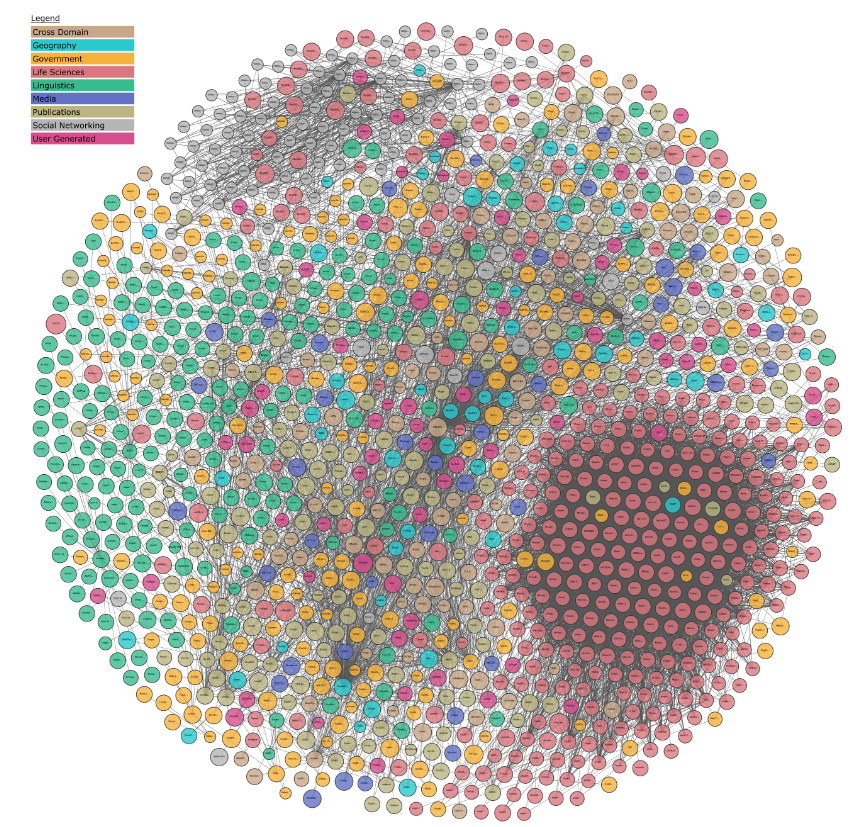
\includegraphics[width=0.8\textwidth]{./chapters/ch-semanticwebpractice/figures/webofdata.png}
	\caption{The linked open data cloud from \textit{lod-cloud.net}.}
	\label{fig:webofdata}
\end{figure}

\subsection{Semantic Search in Semantic Web}

Consider the following query: ``tell me something about Armstrong who landed the eagle on the moon''. Conventionally, the search engine would go through websites, documents, database and other resources, looking for keywords ``Armstrong'', ``landed'', ``eagle'', ``moon''. It will return the sentences or paragraphs that hit most of the matching. This might work. However, it has some drawbacks such as being weak to typo and synonyms.

Semantic search refers to the search of content by meaning, not by keywords. For example, in the context of the increasingly popular LLM, semantic search can be realized using a ``encoder'' (a component in the Transformer) to translate the query to the semantic space. The paragraphs whose semantic space images are close to the query are returned.

In the context of semantic web, semantic search refers to the locating and retrieval of information from the semantic web efficiently based on the query. It is semantic in the sense that the triplestore is able to use logic reasoning during the searching.

In this example, with the semantic web, the search engine interprets ``Armstrong'' not just as a plain word that spells ``a-r-m-s-t-r-o-n-g'', but as a person, ``Neil Armstrong'', with his birthday, birthplace, nationality, etc., all available in one place from his URI (in the case of DBpedia, \textit{https://dbpedia.org/data/Neil\_Armstrong.rdf}). The search engine will understand that ``landing the eagle on the moon'' refers to ``Apollo 11 mission'' as this event is also well defined and has a URI called ``\textit{dbr:Moon\_landing}'' (notice that \textit{dbr} refers to an HTTP URI defined elsewhere). 

Since the semantic web links all the information pieces together, we could have also searched ``tell me something about the first person landed on the moon'' to retrieve everything about ``Neil Armstrong'' all the same, as he can be traced both from his name and from the activities he participated.


















\section{Triplestore}

Triplestore is the database engine of the RDF model. 

When it comes to relational database, there are many choices of DBMS such as Microsoft SQL Server, Oracle DBMS, MySQL and MariaDB. Similarly, there are many choices of triplestores for semantic web. A list of widely used triplestores is given below, just to name a few.
\begin{itemize}
	\item GraphDB: a commercialized enterprise-tier semantic graph database management system compliant with W3C standards. It is famous for its performance and inference capabilities. It also provides free-tier for learning and for small projects, with limited capability.
	\item Apache Jena: an open-source Java framework for building semantic web and linked data applications. It has RDF APIs that can read and process RDF and SPARQL written in XML, Turble, JSON-LD and N-Triples.
	\item Virtuoso: a multi-model DBMS for both RDB and NoSQL databases such as RDF. It is famous for its scalability and standards compliance.
	\item AllegroGraph: a closed source triplestore which is designed to store RDF triples. It also operates as a document store designed for storing, retrieving and managing document-oriented information, in JSON-LD format. AllegroGraph is currently in use in commercial projects and a US Department of Defense project. It offers both free-tier license and enterprise-tier license.
\end{itemize}

More triplestores can be found at W3C, where a list of triplestores is maintained \cite{triplestore,largetriplestore}. As of this writing, there are 50 triplestores registered at W3C.

For the demonstrations given in this notebook, GraphDB is used, unless otherwise mentioned. A full instruction on using GraphDB, including applying for access and installation of the software, can be found at \textit{graphdb.ontotext.com}.

Notice that RDF/RDFS/OWL/SPARQL APIs can be enabled using packages or libraries in many programming languages. For example, in Python, there are several packages available for semantic web operations, including \verb|rdflib|, \verb|Owlready2|, \verb|SPARQLWrapper|, etc. Some of these packages have ``lite'' triplestore engine built-in which provides some SPARQL features for in-memory operations. They do not have all the features of a triplestore. However, they can connect to a triplestore API, in which case they serve as Python-to-triplestore interfaces.


\section{Example: Semantic Web for Home Assets}

As an example, we are creating a semantic web for a the assets in a household. Here ``assets'' refer to the electrical products, furniture, LEGOs, and other non-consumable, relatively static elements. 

We will start with defining classes to divide everything into large groups, including electrical product, furniture, toy, etc. Under each class, sub-classes are defined, such as TV, computer, game console under electrical product, bed, chair, sofa, lamp under furniture, and LEGO under toy. Lastly, we will define instances under each sub-class. For example, bedroom TV and living room TV under TV, Nintendo SWITCH under game console, living room sofa under sofa, study computer, living room computer, TV attached computer under computer, etc.

We will then use RDFS to enforce schema to the RDF model as follows. Consider electrical product class for example. All elements in this class shall have a property called "hasBrand", which maps them to a pre-defined "electricalBrand" class, inside which are commonly seen electrical brands such as Boche, Siemens, Nintendo, Sony, Google, etc. The electrical product shall also have a "hasPrice" property, "warrantyExpiresAt" property, etc. The similar concept applies to all other produces including furniture, etc.

Finally, use OWL to setup some limits of the properties. For example, for electrical products, the price is usually between 0 to 5000 dollars, etc.

The result should be something like Fig. \ref{fig:houseassetexp}, after visualization.

\begin{figure}[htbp]
	\centering
	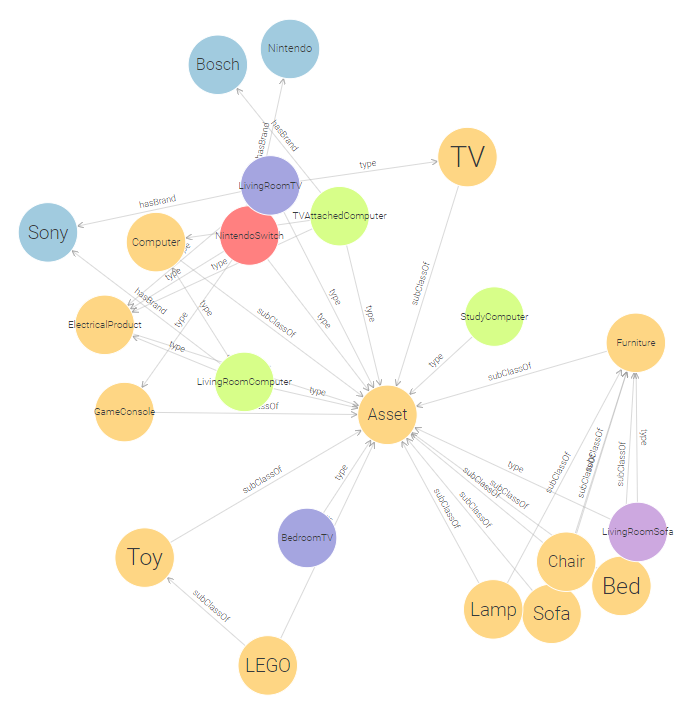
\includegraphics[width=\textwidth]{./chapters/ch-semanticwebpractice/figures/house_asset_exp.png}
	\caption{An example of an RDF model in GraphDB that describes house assets. This is only a demonstration graph and the information inside is artificial and not true.}
	\label{fig:houseassetexp}
\end{figure}

\subsection{Define Classes Hierarchy}

\subsection{Define Properties Hierarchy}

\subsection{Add OWL}

\subsection{Data Retrieval Examples}

\section{Reference: Commonly Used Namespace}

Commonly used built-in name spaces are summarized in Table \ref{tab:commonnamespace}.

\begin{table}
	\centering \caption{Commonly used name spaces in RDF models. URI is neglected since they can be easily found online.} \label{tab:commonnamespace}
	\begin{tabularx}{\textwidth}{lX}
		\hline
		Namespace & Description \\ \hline
		\verb|rdf| & RDF syntax. \\
		\verb|rdfs| & RDFS syntax. \\
		\verb|xsd|  & XML syntax. \\
		\verb|foaf| & Friend-of-a-friend. It describes people, their activities and relations to other people and object. \\
		\hline
	\end{tabularx}
\end{table}

To search URI for a name space, use \textit{prefix.cc}.





























